\section{Introduction}\label{introduction}

Many great semi-empirical methods have been developed over the years to
analyze various aspects of ship hydrodynamics such as: resistance,
propulsion and seakeeping. These methods were often developed because
solving the actual flow was far to complicated and far to time consuming
at the time. When computers are now faster and great advancement in
field of Computation Fluid Dynamics (CFD) has been achieved, the simpler
semi-empirical formulas have now gotten less and less relevant. But have
they all of gotten totally irrelevant?

A semi-empirical method to predict ship roll damping, comonly known as
Ikeda's method, will be investigated in this paper, for a use case that
can still make it relevant. It will be investigated if this method can
be used to increase the accuracy of the roll motion prediction of a
nonlinear potential flow method (FNPF), so that this relatively fast
option can be used to a larger extent than what is currently possible
today. The roll damping of ship is higly depending on vicsous effects
which mean that the invicid potential flow lacks a lot of the important
physics of the roll motion and can therefore not give relevant results
for this degree of freedom, where more advanced options such as: model
test or URANS are needed.

The hybrid method, combining Ikeda's method and FNPF proposed in this
paper is investigated using the well known KVLCC2 test case


\begin{figure}[H]
    \centering
    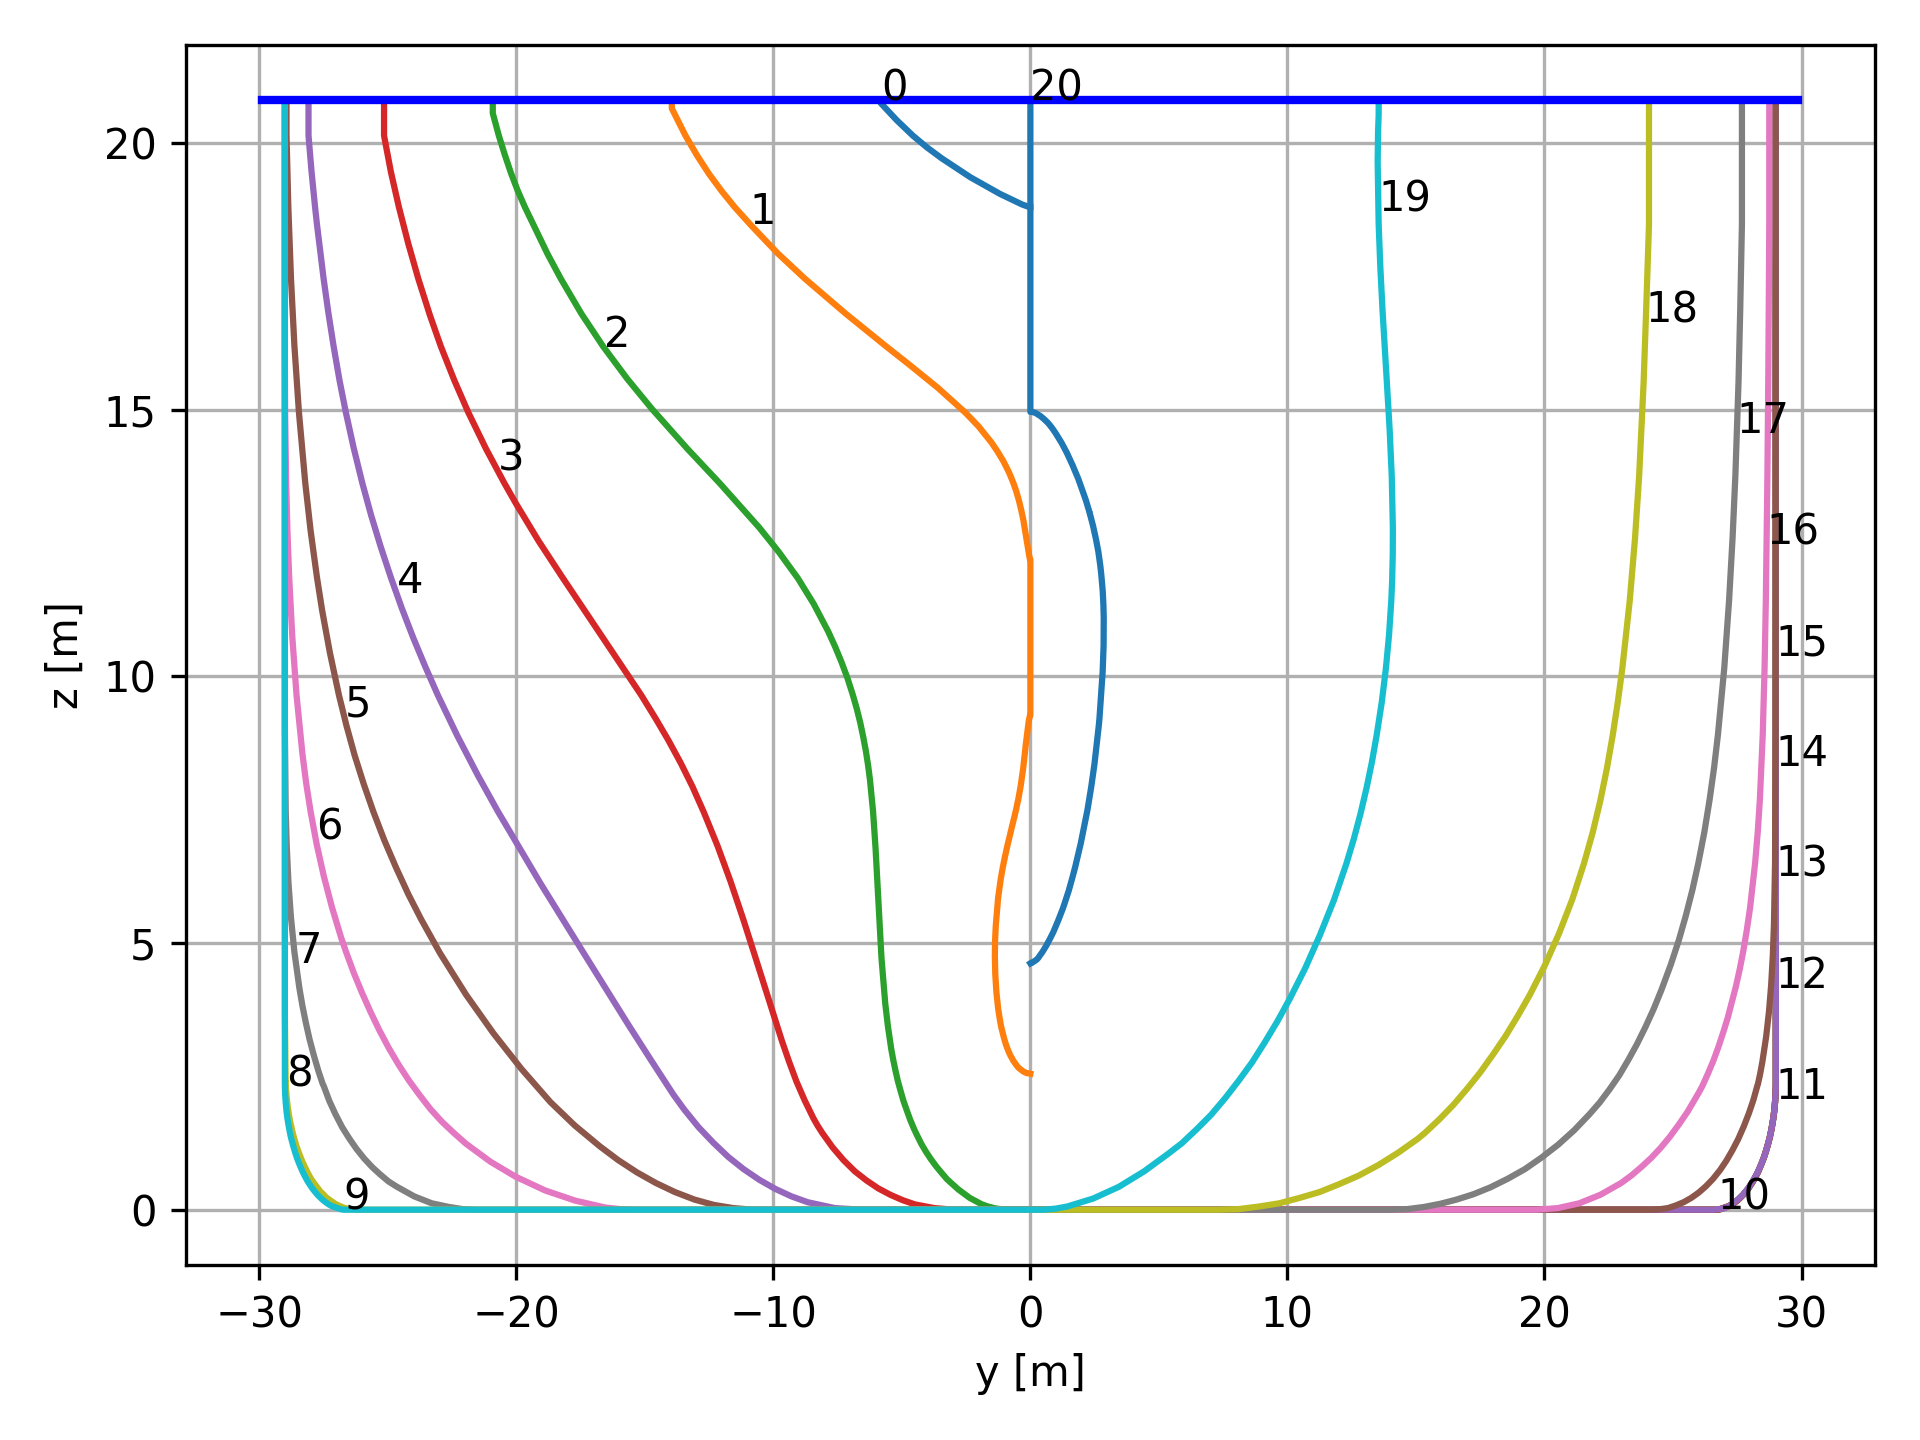
\includegraphics[width=0.9\linewidth]{figures/body_plan.png}
    \caption{Number of tests per ship type}
    \label{fig:ship_types}
    { \hspace*{\fill} \\}
\end{figure}    
 
            
    
    \begin{longtable}[c]{@{}llllllllll@{}}
\toprule\addlinespace
title & LPP & B & ZCG & KXX & S & V & dens & ta & tf\\\addlinespace 
\midrule\endhead
KVLCC2 & 4.706 & 0.853 & 0.274 & 0.341 & 5.981 & 0.993 & 1000.0 & 0.3059 & 0.3059\\\addlinespace 
\bottomrule 
 \end{longtable}

    

    This ship was selected partly because it is a well known test case and
also because it does not have any bilge keels. The Ikeda's metod contain
methods to predict damping from various components, where the bilge
keels is one of them. Results from roll decay test simulations made with
the Hybrid method will be compared to corresponding model test data from
the SSPA Maritime Dynamics Laboratory. From these model tests, only the
total damping can be observed. Reducing the number of components by
having no bilge keels will therefore give more insight into the
remaining components.

Revisiting an older semi-empirical method such as the Ikeda's method can
also be used to gain a deeper understand of the roll damping
hydrodynamics.

    